\documentclass[11pt,a4paper]{article}

% ==================== PAQUETES ====================
\usepackage[spanish]{babel}
\usepackage[utf8]{inputenc}
\usepackage[T1]{fontenc}

\usepackage{geometry}
\geometry{margin=2.5cm}

\usepackage{graphicx}
\usepackage{amsmath}
\usepackage{booktabs}
\usepackage{hyperref}
\usepackage{lmodern}

% opcional: mejor manejo de figuras
\usepackage{float}

% ==================== DATOS ====================
\title{
Título del artículo \\
\large Semillero de Hidrógeno Verde
}

\author{
Autor 1\\
Universidad\\
correo@correo.com
\and
Autor 2\\
Universidad
}

\date{\today}

% ==================== DOCUMENTO ====================
\begin{document}

\maketitle

% ==================== RESUMEN ====================
\begin{abstract}

% 150–250 palabras máximo
% incluir:
% problema
% método
% resultado principal
% impacto en hidrógeno verde

Escribir resumen aquí.

\end{abstract}

\textbf{Palabras clave:} hidrógeno verde, electrólisis, energía renovable, eficiencia

% ==================== INTRODUCCIÓN ====================
\section{Introducción}

% explicar contexto
% por qué el hidrógeno verde es importante
% problema específico del trabajo
% objetivo del artículo

\textbf{Objetivo del trabajo:}

Describir claramente qué se busca analizar o demostrar.

% ==================== MARCO TEÓRICO ====================
\section{Fundamentos Teóricos}

% conceptos necesarios para entender el trabajo
% usar citas si aplica

Ejemplo de eficiencia:

\begin{equation}
\eta = \frac{E_{util}}{E_{entrada}}
\end{equation}

% ejemplos de contenido:
% electrólisis del agua
% energías renovables
% eficiencia energética
% almacenamiento de hidrógeno

% ==================== METODOLOGÍA ====================
\section{Metodología}

% explicar procedimiento
% puede ser:
% experimental
% simulación
% revisión bibliográfica
% modelo matemático

Pasos:

\begin{enumerate}

\item Definir variables del sistema

\item Describir equipo o modelo usado

\item Explicar procedimiento

\item Método de análisis de datos

\end{enumerate}

% ==================== RESULTADOS ====================
\section{Resultados}

% mostrar datos sin interpretar demasiado

\begin{table}[H]
\centering

\begin{tabular}{ccc}

\toprule
Variable & Valor & Unidad \\

\midrule
Ejemplo & 10 & kWh \\
Ejemplo & 5 & kg \\

\bottomrule

\end{tabular}

\caption{Resultados obtenidos}

\end{table}


\begin{figure}[H]

\centering

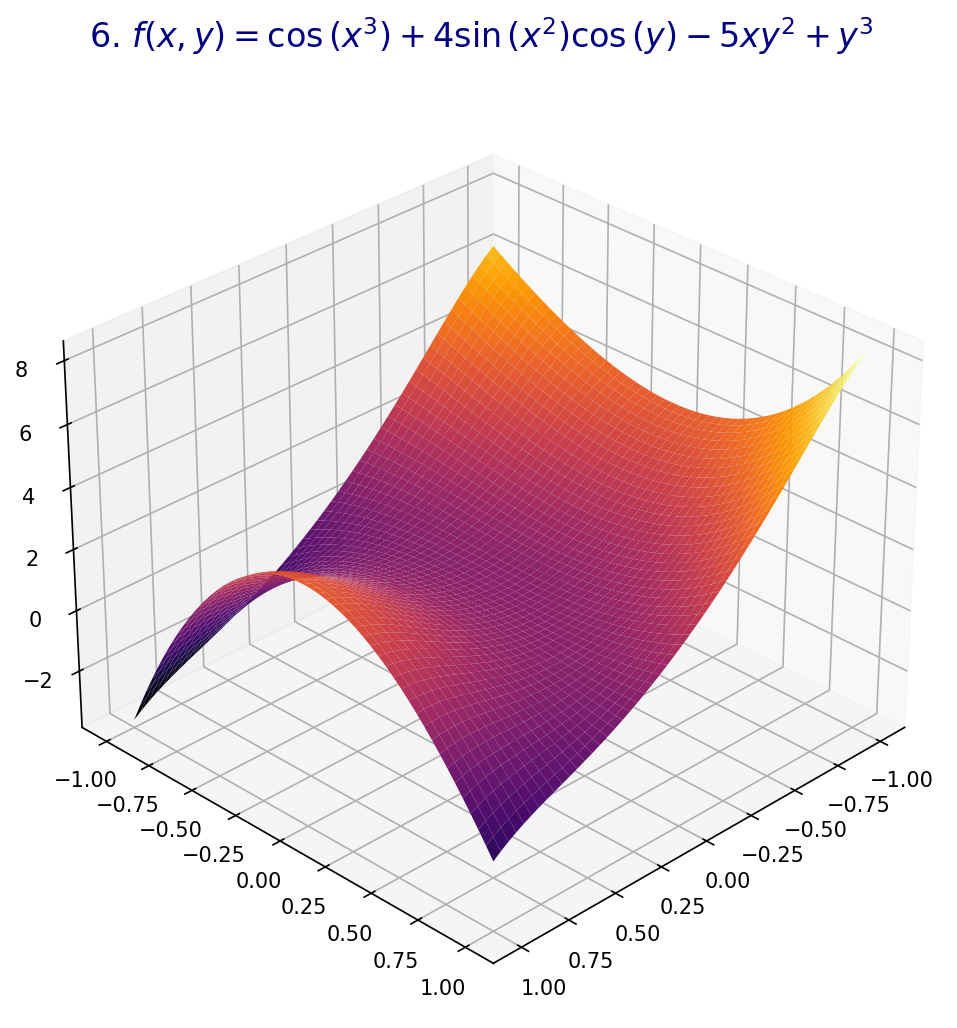
\includegraphics[width=0.75\textwidth]{Imagenes/ejemplo.png}

\caption{Ejemplo de resultado gráfico}

\end{figure}

% ==================== DISCUSIÓN ====================
\section{Discusión}

% interpretar resultados
% comparar con teoría
% explicar posibles errores
% limitaciones del estudio

% ==================== CONCLUSIONES ====================
\section{Conclusiones}

% 3–5 conclusiones claras

\begin{itemize}

\item conclusión principal

\item implicación para hidrógeno verde

\item mejora futura posible

\end{itemize}

% ==================== TRABAJO FUTURO ====================
\section{Trabajo Futuro}

% mejoras posibles
% experimentos adicionales
% aplicaciones industriales

% ==================== REFERENCIAS ====================
\section{Referencias}

% formato simple
% luego puedes migrar a BibTeX si quieres

\begin{enumerate}

\item Autor, título, revista, año.

\item Autor, libro, editorial.

\item DOI o URL.

\end{enumerate}

\end{document}